% !TeX root = ../../Book1.tex
% 纲要标题：### 13.3 Lie 括号与无穷小变换
% 纲要位置：几何学计划纲要.md，第 620 行。
% 正文状态：初稿；尚未正式审核。

% 纲要内容开始
% 
% * 导子交换子与坐标表达
% * 流的交换和 Lie 括号
% * 张量场的 Lie 导数
% * 自然性及分次 Cartan 运算的准备
% 
% 纲要内容结束

\section{Lie 括号与无穷小变换}
\label{g1:sec:1303}

沿两个方向先后运动，交换次序后是否到达同一点？如果两个方向是固定的平面平移，答案是肯定的；如果第二个方向的速度随位置变化，第一步运动就可能改变第二步的效果。这个差别不能只看一点处的两个向量，还要看附近的向量场如何变化。本节把它写成向量场的 Lie 括号，并用流解释这一运算的几何含义。

\ProseParagraphBreak

本节的流形均为有限维、Hausdorff、第二可数、无边界的光滑流形，向量场和张量场均光滑。局部向量场可在其定义开集上应用同样的结果。所需的分析结论是\cref{g1:thm:maximal-local-flow}给出的光滑局部流、流的复合规律及唯一性；不同流的复合总在共同有定义的区域内讨论，不假定向量场完备。

\subsection{导子交换子与坐标表达}
\label{g1:subsec:1303:01}

向量场 \(X\) 作用于一个光滑函数 \(f\)，得到函数 \(Xf\)，其在 \(p\) 的值为 \(X_p(f)\)。由\cref{g1:prop:derivation-coordinate-basis}，在坐标中
\[
	X=\sum_iX^i\partial_i,\qquad Xf=\sum_iX^i\partial_i f,
\]
所以 \(Xf\) 仍光滑，并满足 \(X(fg)=X(f)g+fX(g)\)。这些运算也适用于局部函数：某点附近的函数相等，所得导数在该点附近也相等。于是可以把 \(X\) 看作作用于光滑函数的一个一阶微分算子。

\ProseParagraphBreak

复合算子 \(XY\) 指先作 \(Y\)，再作 \(X\)。它通常包含二阶导数，因而未必还是一个向量场；但是在 \(XY-YX\) 中，二阶部分恰好抵消。

\begin{definition}
	\label{g1:def:lie-bracket}
	设 \(M\) 为无边界光滑流形，\(X,Y\in\mathfrak X(M)\)。定义它们的\term[likuohao]{Lie 括号}[Lie bracket]在局部光滑函数上的作用为
	\[
		[X,Y]f=X(Yf)-Y(Xf).
	\]
	右端是两个算子的交换子。下述计算说明，它确实定义一个光滑向量场，而不只是一个一般微分算子。
\end{definition}

为检查乘法法则，先展开
\[
	XY(fg)=XY(f)\,g+Y(f)X(g)+X(f)Y(g)+f\,XY(g).
\]
交换 \(X,Y\) 后，中间两个交叉项仍是同一对项，相减后得到
\[
	[X,Y](fg)=[X,Y](f)\,g+f[X,Y](g).
\]
因此在每个点，\([X,Y]\) 是函数芽上的导子。按照\cref{g1:prop:derivation-coordinate-basis}，它对应一个切向量，其坐标分量是它作用于坐标函数的值。由 \(Y(x^j)=Y^j\)、\(X(x^j)=X^j\)，得到
\begin{equation}
	\label{g1:eq:lie-bracket-coordinates}
	[X,Y]=\sum_j\left(\sum_iX^i\partial_iY^j-Y^i\partial_iX^j\right)\partial_j.
\end{equation}
系数光滑，故它是光滑向量场。这个坐标表达由无坐标的导子定义推出，所以换坐标时仍表示同一个向量场。

\begin{proposition}[Lie 括号的基本性质]
	\label{g1:prop:lie-bracket-properties}
	设 \(M\) 为无边界光滑流形，\(X,Y,Z\in\mathfrak X(M)\)，\(f,g\in C^\infty(M)\)。Lie 括号对实数双线性，并满足
	\[
		[X,Y]=-[Y,X],\qquad
		[X,[Y,Z]]+[Y,[Z,X]]+[Z,[X,Y]]=0.
	\]
	后一个等式称为 Jacobi 恒等式。此外，
	\begin{equation}
		\label{g1:eq:lie-bracket-product}
		[X,fY]=f[X,Y]+X(f)Y,\qquad
		[fX,gY]=fg[X,Y]+fX(g)Y-gY(f)X.
	\end{equation}
	所有这些等式也适用于同一开集上的局部向量场与函数。
\end{proposition}
\begin{proof}
	实双线性和反对称性直接来自算子复合的分配律。为证明 Jacobi 恒等式，把复合算子作用于任意局部光滑函数，利用复合的结合性展开：
	\[
		\begin{aligned}
			[X,[Y,Z]]&=XYZ-XZY-YZX+ZYX,\\
			[Y,[Z,X]]&=YZX-YXZ-ZXY+XZY,\\
			[Z,[X,Y]]&=ZXY-ZYX-XYZ+YXZ.
		\end{aligned}
	\]
	相加后每个三重复合恰好出现一次正号、一次负号，故总和为零。向量场由它对局部函数的作用确定，所以这是向量场的恒等式。

	对任意局部函数 \(h\)，有
	\[
		[X,fY]h=X(fYh)-fY(Xh)
		=X(f)Yh+f[X,Y]h.
	\]
	这给出第一条乘法公式。再由反对称性得到 \([fX,Y]=f[X,Y]-Y(f)X\)，将第一式用于 \([fX,gY]\)，即得第二式。
\end{proof}

因此 \(\mathfrak X(M)\) 是一个实 Lie 代数，即一个实向量空间，其上配有实双线性括号，且该括号满足反对称性与 Jacobi 恒等式。但括号一般不是对 \(C^\infty(M)\) 双线性的。\eqref{g1:eq:lie-bracket-product}中的函数导数正是区别。比如在平面上，\(X=\partial_x\)、\(Y=x\partial_y\) 满足 \([X,Y]=\partial_y\)。虽然 \(Y\) 在原点为零，括号在原点却不为零；将 \(Y\) 换成恒零向量场，它在原点的值没有改变，括号却变成零。这说明 Lie 括号不是只依赖 \(X_p,Y_p\) 的逐点双线性张量。

\ProseParagraphBreak

坐标场满足 \([\partial_i,\partial_j]=0\)，但任意局部标架没有这一性质。例如 \(e_1=\partial_x\)、\(e_2=e^x\partial_y\) 处处独立，却有 \([e_1,e_2]=e_2\)。已有局部标架并不保证能找到彼此交换的标架，后者还需要一项微分条件；下一节讨论分布时将用到这一区别。

\subsection{流的交换和 Lie 括号}
\label{g1:subsec:1303:02}

令 \(\Phi=\Phi^X\) 为 \(X\) 的最大局部流。回顾\cref{g1:thm:maximal-local-flow}：它定义在含 \(\{0\}\times M\) 的开集 \(\mathcal D_X\subset\mathbb R\times M\) 上，\(\Phi_0=\operatorname{id}\)，并在各项有定义时满足 \(\Phi_{t+s}=\Phi_t\circ\Phi_s\)。固定 \(t\) 后，\(\Phi_t\) 是其开定义域与像之间的微分同胚，逆为 \(\Phi_{-t}\)。这些性质允许我们把不同点的向量带到同一个切空间中比较。

\ProseParagraphBreak

直接求 \(Y_{\Phi_t(p)}-Y_p\) 没有内在意义，因为两个向量的基点不同。应先用逆流的微分将第一个向量带回 \(\mathrm{T}_pM\)，定义
\begin{equation}
	\label{g1:eq:flow-vector-pullback}
	\bigl((\Phi_t)^*Y\bigr)_p
	=\mathrm{d}(\Phi_{-t})_{\Phi_t(p)}Y_{\Phi_t(p)}
	=\bigl(\mathrm{d}(\Phi_t)_p\bigr)^{-1}Y_{\Phi_t(p)}.
\end{equation}
这是\cref{g1:prop:mixed-tensor-pullback}的向量场拉回。对函数则是 \((\Phi_t)^*f=f\circ\Phi_t\)。拉回先移动观察点，再将该点的几何量搬回原点，所以其变化率同时记录向量场和搬运方式的变化。

\begin{proposition}[沿流的拉回导数]
	\label{g1:prop:flow-pullback-derivative}
	设 \(M\) 为无边界光滑流形，\(X,Y\in\mathfrak X(M)\)，\(\Phi\) 为 \(X\) 的局部流。则在共同有定义的区域内，
	\[
		\left.\frac{\mathrm{d}}{\mathrm{d}t}\right|_{t=0}(\Phi_t)^*Y=[X,Y],
		\qquad
		\frac{\mathrm{d}}{\mathrm{d}t}(\Phi_t)^*Y
		=(\Phi_t)^*[X,Y]=[X,(\Phi_t)^*Y].
	\]
	对任意光滑函数 \(f\)，还有
	\[
		\frac{\mathrm{d}}{\mathrm{d}t}(\Phi_t)^*f=(\Phi_t)^*(Xf).
	\]
	特别地，\([X,Y]=0\) 当且仅当 \(Y\) 被 \(X\) 的局部流保持，即 \((\Phi_t)^*Y=Y\)；等价地，
	\[
		\mathrm{d}(\Phi_t)_pY_p=Y_{\Phi_t(p)}
	\]
	在流的定义域内成立。
\end{proposition}
\begin{proof}
	先在一点附近选坐标，把 \(X,Y\) 的分量视为列向量，流的坐标表达记为 \(\phi_t(x)\)。由\cref{g1:thm:ode-smooth-dependence}的光滑依赖及流方程，
	\[
		\phi_0(x)=x,\qquad
		\left.\partial_t\phi_t(x)\right|_0=X(x),\qquad
		\left.\partial_t\mathrm{D}\phi_t(x)\right|_0=\mathrm{D}X(x).
	\]
	记 \(A(t)=\mathrm{D}\phi_t(x)\)。对 \(A(t)^{-1}A(t)=I\) 求导，并用 \(A(0)=I\)，得到 \((A^{-1})'(0)=-\mathrm{D}X(x)\)。因此\eqref{g1:eq:flow-vector-pullback}的导数为
	\[
		\left.\frac{\mathrm{d}}{\mathrm{d}t}\right|_0
		\bigl(\mathrm{D}\phi_t(x)^{-1}Y(\phi_t(x))\bigr)
		=-\mathrm{D}X(x)Y(x)+\mathrm{D}Y(x)X(x).
	\]
	第 \(j\) 个分量正是\eqref{g1:eq:lie-bracket-coordinates}的系数，证明了零时刻公式。

	固定一个有定义的 \((t,p)\)。由流定义域的开放性，在 \(p\) 的适当邻域及 \(h=0\) 附近，可同时使用
	\[
		(\Phi_{t+h})^*=(\Phi_t)^*(\Phi_h)^*
		=(\Phi_h)^*(\Phi_t)^*.
	\]
	第一种分解对 \(h\) 求导，得到 \((\Phi_t)^*[X,Y]\)；第二种分解把 \((\Phi_t)^*Y\) 视为局部向量场，使用已经证明的零时刻公式，得到 \([X,(\Phi_t)^*Y]\)。函数公式则直接由沿积分曲线的链式法则得到。

	若 \([X,Y]=0\)，固定 \(p\) 后，上述拉回在包含零的时间定义区间内导数为零。它始终位于固定的向量空间 \(\mathrm{T}_pM\)，按任意基逐分量应用一元微积分，便知它恒等于零时刻的 \(Y_p\)。反之，拉回保持不变时在零时刻求导，得到括号为零。最后一个等式由乘以可逆的 \(\mathrm{d}(\Phi_t)_p\) 得到。
\end{proof}

公式中的负号来自逆微分的求导，不能只沿轨道对 \(Y\) 的分量求导而略去它。另一个直接的检验是 \(X\) 自己被其流保持：对 \(\Phi_t(\Phi_s(p))=\Phi_{t+s}(p)\) 在 \(s=0\) 求导，得到 \(\mathrm{d}(\Phi_t)_pX_p=X_{\Phi_t(p)}\)，与 \([X,X]=0\) 一致。

\begin{theorem}[交换的局部流]
	\label{g1:thm:commuting-local-flows}
	设 \(M\) 为无边界光滑流形，\(X,Y\in\mathfrak X(M)\)，局部流分别为 \(\Phi,\Psi\)。以下两项等价：
	\begin{enumerate}
		\item \([X,Y]=0\)。
		\item 对每个 \(p\in M\)，存在开邻域 \(U\) 和 \(\varepsilon>0\)，使对所有 \(q\in U\) 及 \(|s|,|t|<\varepsilon\)，两种复合均有定义且
		\[
			\Phi_t(\Psi_s(q))=\Psi_s(\Phi_t(q)).
		\]
	\end{enumerate}
	这里不要求两向量场完备，结论是共同定义域内的局部交换。
\end{theorem}
\begin{proof}
	假设括号为零。两个复合映射的定义条件各自在 \(\mathbb R^2\times M\) 中构成开集，并且都包含 \((0,0,p)\)：这是因为各流定义域开，且中间点随参数连续变化。取这两个开集交中的一个乘积邻域 \((-\varepsilon,\varepsilon)^2\times U\)，便得到陈述中统一的共同定义域。

	固定 \(q\in U\) 及 \(|t|<\varepsilon\)。由于 \(X\) 的流保持 \(Y\)，曲线 \(c(s)=\Phi_t(\Psi_s(q))\) 满足
	\[
		c'(s)=\mathrm{d}(\Phi_t)_{\Psi_s(q)}Y_{\Psi_s(q)}
		=Y_{c(s)},\qquad c(0)=\Phi_t(q).
	\]
	曲线 \(s\mapsto\Psi_s(\Phi_t(q))\) 也满足同一个初值问题。积分曲线唯一性使它们在 \((-\varepsilon,\varepsilon)\) 上相同，故两种流交换。

	反过来，假设第二项成立。将交换式对 \(s\) 在零处求导，得到
	\[
		\mathrm{d}(\Phi_t)_qY_q=Y_{\Phi_t(q)}.
	\]
	所以 \((\Phi_t)^*Y=Y\) 在相应邻域和小时间上成立。再对 \(t\) 在零处求导，由\cref{g1:prop:flow-pullback-derivative}得到 \([X,Y]_q=0\)。每个点都有这样的邻域，故括号处处为零。
\end{proof}

\begin{example}[运动次序的差别]
	\label{g1:exm:noncommuting-plane-flows}
	在 \(\mathbb R^2\) 上取 \(X=\partial_x\)、\(Y=x\partial_y\)。它们的流在所有时间有定义：
	\[
		\Phi_t(x,y)=(x+t,y),\qquad
		\Psi_s(x,y)=(x,y+sx).
	\]
	两种次序分别得到
	\[
		\Phi_t\Psi_s(x,y)=(x+t,y+sx),\qquad
		\Psi_s\Phi_t(x,y)=(x+t,y+s(x+t)).
	\]
	第二个终点比第一个多出竖直位移 \(st\)，如\cref{g1:fig:flow-order}所示。原因是先沿 \(X\) 移动会增大随后沿 \(Y\) 运动的速度；而先沿 \(Y\) 运动时，这个增大尚未发生。括号 \([X,Y]=\partial_y\) 正好指出这个差别的方向。沿 \(X\) 的拉回也能直接看到它：\((\Phi_t)^*Y=(x+t)\partial_y\)，对 \(t\) 求导得到 \(\partial_y\)。
\end{example}

% !TeX root = ../Book1.tex
\begin{figure}[htbp]
	\centering
	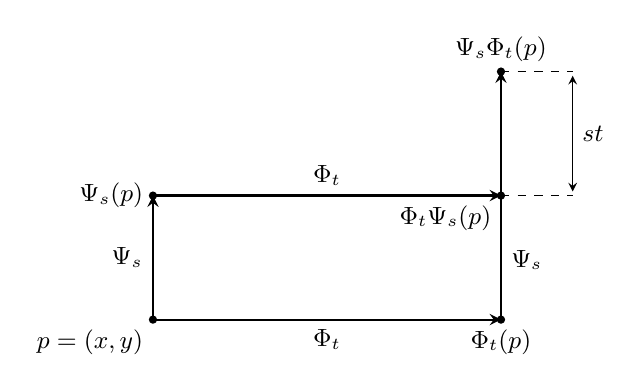
\begin{tikzpicture}[>=stealth,x=1.3cm,y=1.05cm,font=\small]
		\coordinate (P) at (0,0);
		\coordinate (XP) at (3.4,0);
		\coordinate (YP) at (0,1.5);
		\coordinate (XYP) at (3.4,1.5);
		\coordinate (YXP) at (3.4,3);
		\draw[->,thick] (P)--node[below] {\(\Phi_t\)} (XP);
		\draw[->,thick] (P)--node[left] {\(\Psi_s\)} (YP);
		\draw[->,thick] (YP)--node[above] {\(\Phi_t\)} (XYP);
		\draw[->,thick] (XP)--node[right,pos=.24] {\(\Psi_s\)} (YXP);
		\draw[dashed] (XYP)--(4.1,1.5);
		\draw[dashed] (YXP)--(4.1,3);
		\draw[<->] (4.1,1.55)--node[right] {\(st\)} (4.1,2.95);
		\foreach \Q in {P,XP,YP,XYP,YXP} \fill (\Q) circle (1.5pt);
		\node[below left] at (P) {\(p=(x,y)\)};
		\node[below] at (XP) {\(\Phi_t(p)\)};
		\node[left] at (YP) {\(\Psi_s(p)\)};
		\node[below left] at (XYP) {\(\Phi_t\Psi_s(p)\)};
		\node[above] at (YXP) {\(\Psi_s\Phi_t(p)\)};
	\end{tikzpicture}
	\caption{\(X=\partial_x\)、\(Y=x\partial_y\) 的两种运动次序，图中以 \(x,s,t>0\) 示意。先作水平运动会增加随后竖直运动的速度，两个终点的竖直差为 \(st\)。}
	\label{g1:fig:flow-order}
\end{figure}


\subsection{张量场的 Lie 导数}
\label{g1:subsec:1303:03}

流不仅可以搬运向量，也可以搬运度量、形式以及其他张量。\cref{g1:prop:mixed-tensor-pullback}已经说明，微分同胚拉回一个 \((r,s)\) 型张量时，对每个向量因子使用逆微分，对每个对偶因子使用微分的对偶。因此对 \(X\) 的流 \(\Phi\)，
\[
	\bigl((\Phi_t)^*T\bigr)_p
	=\left(\bigl(\mathrm{d}(\Phi_t)_p\bigr)^{-1}\right)^{\otimes r}
	\otimes\left(\bigl(\mathrm{d}(\Phi_t)_p\bigr)^*\right)^{\otimes s}
	\bigl(T_{\Phi_t(p)}\bigr).
\]
这个表达始终位于 \(T^r_s(\mathrm{T}_pM)\)，可以在固定纤维中对时间求导。

\begin{definition}
	\label{g1:def:lie-derivative-tensor}
	设 \(M\) 为无边界光滑流形，\(X\in\mathfrak X(M)\)，\(T\) 为光滑 \((r,s)\) 型张量场。定义 \(T\) 沿 \(X\) 的\term[lidaoshu]{Lie 导数}[Lie derivative]为
	\[
		\mathcal L_XT=\left.\frac{\mathrm{d}}{\mathrm{d}t}\right|_{t=0}(\Phi_t^X)^*T.
	\]
	导数在各点固定的张量纤维中取。局部流对时间和初值光滑，张量拉回的局部公式也光滑，因此这一定义给出同型的光滑张量场。
\end{definition}

在函数上有 \(\mathcal L_Xf=Xf\)，在向量场上有 \(\mathcal L_XY=[X,Y]\)。所以 Lie 导数扩展了同一个沿流比较的想法，无需另选内积或联络；它比较的方式由 \(X\) 的流本身确定。

\begin{proposition}[张量 Lie 导数的计算]
	\label{g1:prop:lie-derivative-tensor-rules}
	设 \(M\) 为无边界光滑流形，\(X\in\mathfrak X(M)\)，\(T,S\) 为光滑张量场，\(f\) 为光滑函数。Lie 导数实线性，并满足
	\[
		\mathcal L_X(T\otimes S)=(\mathcal L_XT)\otimes S+T\otimes(\mathcal L_XS),\qquad
		\mathcal L_X(fT)=X(f)T+f\mathcal L_XT.
	\]
	对任意指定位置的收缩 \(C\)，有 \(\mathcal L_X(CT)=C(\mathcal L_XT)\)。在局部坐标中，
	\begin{equation}
		\label{g1:eq:lie-derivative-tensor-coordinates}
		\begin{split}
			(\mathcal L_XT)^{i_1\cdots i_r}{}_{j_1\cdots j_s}
			={}&\sum_kX^k\partial_kT^{i_1\cdots i_r}{}_{j_1\cdots j_s}\\
			&-\sum_{a=1}^r\sum_k(\partial_kX^{i_a})
			T^{i_1\cdots i_{a-1}k i_{a+1}\cdots i_r}{}_{j_1\cdots j_s}\\
			&+\sum_{b=1}^s\sum_k(\partial_{j_b}X^k)
			T^{i_1\cdots i_r}{}_{j_1\cdots j_{b-1}k j_{b+1}\cdots j_s}.
		\end{split}
	\end{equation}
	此外，在流的共同定义域内，
	\[
		\frac{\mathrm{d}}{\mathrm{d}t}(\Phi_t^X)^*T
		=(\Phi_t^X)^*(\mathcal L_XT)
		=\mathcal L_X\bigl((\Phi_t^X)^*T\bigr).
	\]
	因此 \(\mathcal L_XT=0\) 当且仅当 \(T\) 被 \(X\) 的局部流保持。
\end{proposition}
\begin{proof}
	拉回保持张量积与收缩，见\cref{g1:prop:mixed-tensor-pullback}。对这些恒等式在 \(t=0\) 求导，用通常的乘积求导法则，便得到前两条乘法公式及收缩相容性。它也保持因子的排列，因此对称张量和交替张量的 Lie 导数仍保持各自的对称性。

	为得到坐标公式，先计算坐标基及对偶基的导数。向量场情形已知
	\[
		\mathcal L_X\partial_i=[X,\partial_i]=-\sum_k(\partial_iX^k)\partial_k.
	\]
	对任意一形式 \(\alpha\) 与向量场 \(Y\)，拉回和求值相容：
	\[
		(\Phi_t)^*(\alpha(Y))=((\Phi_t)^*\alpha)((\Phi_t)^*Y).
	\]
	在零时刻求导，得到
	\begin{equation}
		\label{g1:eq:lie-one-form-evaluation}
		(\mathcal L_X\alpha)(Y)=X(\alpha(Y))-\alpha([X,Y]).
	\end{equation}
	令 \(\alpha=\mathrm{d}x^j\)、\(Y=\partial_i\)，由于 \(\mathrm{d}x^j(\partial_i)=\delta_i^j\) 为常数，便有
	\[
		\mathcal L_X(\mathrm{d}x^j)=\sum_i(\partial_iX^j)\,\mathrm{d}x^i.
	\]
	将 \(T\) 在坐标张量基中展开，分别对系数、每个向量基因子及每个对偶基因子求导，就得到\eqref{g1:eq:lie-derivative-tensor-coordinates}。上指标的负号来自向量基的导数，下指标的正号来自对偶基的导数。

	最后，与\cref{g1:prop:flow-pullback-derivative}的证明一样，在一个共同定义的邻域中分别用
	\[
		(\Phi_{t+h})^*=(\Phi_t)^*(\Phi_h)^*
		=(\Phi_h)^*(\Phi_t)^*
	\]
	对 \(h\) 在零处求导，得到一般时间的两个等式。若 \(\mathcal L_XT=0\)，固定 \(p\) 后，\(\bigl((\Phi_t)^*T\bigr)_p\) 在固定有限维张量空间中导数为零，故等于 \(T_p\)；反向只需在 \(t=0\) 求导。
\end{proof}

同样对一般求值恒等式求导，可以得到一个无需坐标的计算方法。若 \(T\) 为协变 \(k\) 阶张量，则
\begin{equation}
	\label{g1:eq:lie-covariant-evaluation}
	(\mathcal L_XT)(Y_1,\ldots,Y_k)
	=X\bigl(T(Y_1,\ldots,Y_k)\bigr)
	-\sum_{a=1}^kT(Y_1,\ldots,[X,Y_a],\ldots,Y_k).
\end{equation}
右端第一项对整个实值函数求导，后面的各项扣除输入向量场随流变化的影响。对混合张量，还要对每个协变向量输入扣除对应的 \(\mathcal L_X\alpha\) 项；这由相同的求值乘积法则得到。只保留第一个方向导数而省略输入的修正，一般不会得到张量运算。

\begin{example}[膨胀下的张量变化]
	\label{g1:exm:lie-dilation-tensors}
	在 \(\mathbb R^n\) 上令 \(X=\sum_i x^i\partial_i\)，其流为 \(\Phi_t(x)=e^t x\)。常向量场和坐标一形式的拉回分别满足
	\[
		(\Phi_t)^*\partial_i=e^{-t}\partial_i,\qquad
		(\Phi_t)^*(\mathrm{d}x^i)=e^t\,\mathrm{d}x^i.
	\]
	所以 \(\mathcal L_X\partial_i=-\partial_i\)，而 \(\mathcal L_X(\mathrm{d}x^i)=\mathrm{d}x^i\)。Euclid 内积与标准最高次形式因而满足
	\[
		\mathcal L_X\left(\sum_i\mathrm{d}x^i\otimes\mathrm{d}x^i\right)
		=2\sum_i\mathrm{d}x^i\otimes\mathrm{d}x^i,\qquad
		\mathcal L_X(\mathrm{d}x^1\wedge\cdots\wedge\mathrm{d}x^n)
		=n\,\mathrm{d}x^1\wedge\cdots\wedge\mathrm{d}x^n.
	\]
	这些张量的坐标系数都是常数，Lie 导数却不为零，因为膨胀会改变向量输入的尺度。相反，对任意常数倍平移场，流的微分是恒等映射，这些常系数张量的 Lie 导数为零。
\end{example}

\subsection{自然性及分次 Cartan 运算的准备}
\label{g1:subsec:1303:04}

讨论映射与 Lie 括号的相容性时，不能沿任意光滑映射直接“推出一个向量场”。微分确实把单个切向量向前送，但同一目标点可能有多个原像，得到的向量未必一致；也可能目标方向根本不在微分的像中。需要明确要求两边的场彼此对应。

\begin{definition}
	\label{g1:def:related-vector-fields}
	设 \(F:M\to N\) 为无边界光滑流形之间的光滑映射。若 \(X\in\mathfrak X(M)\)、\(\overline X\in\mathfrak X(N)\) 满足
	\[
		\mathrm{d}F_pX_p=\overline X_{F(p)}\qquad(p\in M),
	\]
	称它们为 \(F\)-\term[xiangguanxiangliangchang]{相关向量场}[related vector fields]。
\end{definition}

由\cref{g1:def:manifold-differential}，相关条件等价于对目标上的每个局部光滑函数 \(f\) 有
\[
	X(f\circ F)=(\overline Xf)\circ F.
\]
反向也成立，因为将这一等式用于目标坐标函数，就能逐分量确定两个目标切向量相等。因此相关条件可以用函数检验，无需给 \(F\) 额外的可逆性。

\begin{proposition}[Lie 导数的自然性]
	\label{g1:prop:lie-derivative-natural}
	设 \(F:M\to N\) 为无边界光滑流形之间的光滑映射，\(X,\overline X\) 为 \(F\)-相关向量场。
	\begin{enumerate}
		\item 若 \(Y,\overline Y\) 也 \(F\)-相关，则 \([X,Y]\) 与 \([\overline X,\overline Y]\) \(F\)-相关。
		\item 记 \(X,\overline X\) 的局部流为 \(\Phi,\overline\Phi\)，则在每个初始点附近的充分小共同时间内，
		\[
			F\circ\Phi_t=\overline\Phi_t\circ F.
		\]
		\item 对 \(N\) 上任意光滑协变张量 \(T\)，有
		\[
			\mathcal L_X(F^*T)=F^*(\mathcal L_{\overline X}T).
		\]
		若 \(F\) 为局部微分同胚，同式也适用于任意混合张量。对任意微分形式 \(\alpha\)，无须可逆性即有
		\[
			\iota_X(F^*\alpha)=F^*(\iota_{\overline X}\alpha).
		\]
	\end{enumerate}
\end{proposition}
\begin{proof}
	对任意目标局部函数 \(f\)，连续使用相关条件可得
	\[
		\begin{aligned}
			[X,Y](f\circ F)
			&=X\bigl((\overline Yf)\circ F\bigr)
			-Y\bigl((\overline Xf)\circ F\bigr)\\
			&=(\overline X\overline Yf-\overline Y\overline Xf)\circ F
			=([\overline X,\overline Y]f)\circ F.
		\end{aligned}
	\]
	由函数检验条件得到第一项。这里既没有使用单射性，也没有使用满射性。

	对固定 \(p\)，曲线 \(t\mapsto F(\Phi_t(p))\) 的导数为
	\[
		\mathrm{d}F_{\Phi_t(p)}X_{\Phi_t(p)}
		=\overline X_{F(\Phi_t(p))},
	\]
	初值为 \(F(p)\)。它与 \(t\mapsto\overline\Phi_t(F(p))\) 满足同一初值问题，故在共同时间内相同。局部流的开定义域和连续性允许在 \(p\) 的一个邻域中同时选取充分小的时间区间，得到第二项的局部映射恒等式。

	协变张量的拉回始终有定义，并与复合相容，见\cref{g1:prop:covariant-tensor-pullback}。将第二项拉回，得到
	\[
		\Phi_t^*(F^*T)=F^*(\overline\Phi_t^*T).
	\]
	对 \(t\) 在零处求导，得到第三项的 Lie 导数公式。右边的 \(F^*\) 由固定的微分 \(\mathrm{d}F\) 作用于各输入，局部表达是固定系数与张量分量的有限次乘法和求和，所以求导可以穿过它。若 \(F\) 为局部微分同胚，各微分可逆，\cref{g1:prop:mixed-tensor-pullback}使同一个论证也适用于混合张量。

	最后，对任意 \(v_1,\ldots,v_{k-1}\in \mathrm{T}_pM\)，有
	\[
		\begin{aligned}
			\bigl(\iota_XF^*\alpha\bigr)_p(v_1,\ldots,v_{k-1})
			&=\alpha_{F(p)}(\mathrm{d}F_pX_p,\mathrm{d}F_pv_1,\ldots,\mathrm{d}F_pv_{k-1})\\
			&=\alpha_{F(p)}(\overline X_{F(p)},\mathrm{d}F_pv_1,\ldots,\mathrm{d}F_pv_{k-1}),
		\end{aligned}
	\]
	恰为右端的值。零次形式时两边均为零。
\end{proof}

若 \(F\) 是微分同胚，可以定义目标向量场
\[
	(F_*X)_q=\mathrm{d}F_{F^{-1}(q)}X_{F^{-1}(q)}.
\]
此时相关性自动成立，命题给出 \(F_*[X,Y]=[F_*X,F_*Y]\)。但对于投影 \(P(x,y)=x\)，向量场 \(y\partial_x\) 在不同原像 \((x,y)\) 上会送出不同的目标速度，因此没有与它相关的目标向量场。自然性命题的假设不能由“映射光滑”代替。

\ProseParagraphBreak

最后整理微分形式上的两个运算。\(\mathcal L_X\) 保持形式次数，\(\iota_X\) 将次数降低 \(1\)，并在函数上取零。\cref{g1:prop:interior-product-rule}已经证明
\[
	\iota_X(\alpha\wedge\beta)
	=(\iota_X\alpha)\wedge\beta+(-1)^p\alpha\wedge(\iota_X\beta),
	\qquad \alpha\in\Omega^p(M).
\]
符号来自将被插入的向量越过前面 \(p\) 个输入位置。把这类带次数的运算放在一起时，合适的交换子是
\[
	[A,B]_{\mathrm{gr}}=A\circ B-(-1)^{ab}B\circ A,
\]
其中 \(a,b\) 是各自改变形式次数的数。这称为分次交换子；两个次数为 \(-1\) 的运算之间对应的是反交换和，而不是普通差。

\begin{proposition}[插入与 Lie 导数]
	\label{g1:prop:cartan-insertion-identities}
	设 \(M\) 为无边界光滑流形，\(X,Y\in\mathfrak X(M)\)，\(\alpha,\beta\) 为微分形式。则
	\[
		\mathcal L_X(\alpha\wedge\beta)
		=(\mathcal L_X\alpha)\wedge\beta+\alpha\wedge(\mathcal L_X\beta),
	\]
	并且
	\begin{align*}
		\iota_X\iota_Y+\iota_Y\iota_X&=0,\\
		\mathcal L_X\iota_Y-\iota_Y\mathcal L_X&=\iota_{[X,Y]},\\
		\mathcal L_X\mathcal L_Y-\mathcal L_Y\mathcal L_X&=\mathcal L_{[X,Y]}.
	\end{align*}
	最后一式也适用于任意混合张量场。
\end{proposition}
\begin{proof}
	拉回保持楔积，故对 \(\Phi_t^*(\alpha\wedge\beta)=\Phi_t^*\alpha\wedge\Phi_t^*\beta\) 在零时刻求导，得到第一式。Lie 导数的次数是零，因此第二项前没有额外的分次符号。

	对至少二次的形式 \(\alpha\)，先插入 \(Y\)，再插入 \(X\)，得到
	\[
		(\iota_X\iota_Y\alpha)(v_1,\ldots)=\alpha(Y,X,v_1,\ldots).
	\]
	反向次序给出 \(\alpha(X,Y,v_1,\ldots)\)，由交替性二者相加为零。次数为零或一时，两次插入都给出零，因此第一条交换关系对所有次数成立。

	取 \(X\) 的局部流 \(\Phi\)。\cref{g1:prop:lie-derivative-natural}的插入相容性用于微分同胚 \(\Phi_t\)，其中源向量场是 \(\Phi_t^*Y\)，得到
	\[
		\Phi_t^*(\iota_Y\alpha)
		=\iota_{\Phi_t^*Y}(\Phi_t^*\alpha).
	\]
	插入对向量场和形式各自线性，且逐点为双线性运算。对右端用乘积求导法则，并用 \(\left.\partial_t\right|_0\Phi_t^*Y=[X,Y]\)，便得
	\[
		\mathcal L_X(\iota_Y\alpha)
		=\iota_{[X,Y]}\alpha+\iota_Y(\mathcal L_X\alpha),
	\]
	这就是第二条交换关系。

	为证明最后一条，记 \(D=\mathcal L_X\mathcal L_Y-\mathcal L_Y\mathcal L_X-\mathcal L_{[X,Y]}\)。两个次数为零的张量积导子的交换子仍是张量积导子：将它作用于 \(T\otimes S\)，展开后交叉项 \((\mathcal L_XT)\otimes(\mathcal L_YS)\) 与 \((\mathcal L_YT)\otimes(\mathcal L_XS)\) 分别抵消，余下的正是两端各自求导之和。因此 \(D\) 是张量积导子，并且与收缩相容。

	在函数上，\(Df=XYf-YXf-[X,Y]f=0\)。在向量场 \(Z\) 上，由 Jacobi 恒等式，
	\[
		DZ=[X,[Y,Z]]-[Y,[X,Z]]-[[X,Y],Z]=0.
	\]
	对任意一形式 \(\eta\) 与局部向量场 \(Z\)，求值是张量积之后的收缩，所以
	\[
		0=D(\eta(Z))=(D\eta)(Z)+\eta(DZ)=(D\eta)(Z).
	\]
	取坐标向量场逐个检验，得到 \(D\eta=0\)。任意张量在局部都是光滑函数乘若干向量场与一形式的张量积之和，导子法则遂给出 \(DT=0\)。这证明了所有混合张量上的最后一式，形式情形包含在其中。
\end{proof}

这些等式把运动、插入和交替性联系起来。在\secref{g1:sec:1401}中，将构造把形式次数提高 \(1\) 的外微分 \(\mathrm{d}\)，并证明 Cartan 公式\footnote{Cartan，Élie Joseph Cartan（1869--1951），法国数学家，研究 Lie 群、Lie 代数与微分几何，发展了活动标架方法。}
\[
	\mathcal L_X=\mathrm{d}\iota_X+\iota_X\mathrm{d}.
\]
这里的加号与两个奇次数运算的分次交换子相符；定义外微分以后，将给出该公式及其证明。
% 纲要条目排为编号小节标题，并进入目录与书签；说明段仍保留于纲要注释中。
